% mnras_guide.tex
%
% MNRAS LaTeX user guide
%
% v3.1 released 11 June 2020
%
% v3.0 released 22 May 2015
% (version numbers match those of mnras.cls)
%
% Copyright (C) Royal Astronomical Society 2015
% Authors:
% Keith T. Smith (Royal Astronomical Society)

% Change log
%
% v3.0   September 2013 - May 2015
%    First version: complete rewrite of the user guide
%    Basic structure taken from mnras_template.tex by the same author

%%%%%%%%%%%%%%%%%%%%%%%%%%%%%%%%%%%%%%%%%%%%%%%%%%
% Basic setup. Most papers should leave these options alone.
\documentclass[fleqn,usenatbib,useAMS]{mnras}

%%%%% AUTHORS - PLACE YOUR OWN PACKAGES HERE %%%%%

% Only include extra packages if you really need them. Common packages are:
\usepackage{graphicx}	% Including figure files
\usepackage{amsmath}	% Advanced maths commands
\usepackage{amssymb}	% Extra maths symbols
\usepackage{multicol}        % Multi-column entries in tables
\usepackage{bm}		% Bold maths symbols, including upright Greek
\usepackage{pdflscape}	% Landscape pages

%%%%%%%%%%%%%%%%%%%%%%%%%%%%%%%%%%%%%%%%%%%%%%%%%%

%%%%%% AUTHORS - PLACE YOUR OWN MACROS HERE %%%%%%

% Please keep new commands to a minimum, and use \newcommand not \def to avoid
% overwriting existing commands. Example:
%\newcommand{\pcm}{\,cm$^{-2}$}	% per cm-squared
\newcommand{\kms}{\,km\,s$^{-1}$} % kilometres per second
\newcommand{\bibtex}{\textsc{Bib}\!\TeX} % bibtex. Not quite the correct typesetting, but close enough

%%%%%%%%%%%%%%%%%%%%%%%%%%%%%%%%%%%%%%%%%%%%%%%%%%


% Use vector fonts, so it zooms properly in on-screen viewing software
% Don't change these lines unless you know what you are doing
\usepackage[T1]{fontenc}
\usepackage{ae,aecompl}

% MNRAS is set in Times font. If you don't have this installed (most LaTeX
% installations will be fine) or prefer the old Computer Modern fonts, comment
% out the following line
\usepackage{newtxtext,newtxmath}
% Depending on your LaTeX fonts installation, you might get better results with one of these:
%\usepackage{mathptmx}
%\usepackage{txfonts}

%%%%%%%%%%%%%%%%%%% TITLE PAGE %%%%%%%%%%%%%%%%%%%

% Title of the paper, and the short title which is used in the headers.
% Keep the title short and informative.
	\title[Kalman PTA]{State-space PTA}

% The list of authors, and the short list which is used in the headers.
% If you need two or more lines of authors, add an extra line using \newauthor
\author[Kimpson]{Kimpson$^{1}$, O'Leary, Melatos, Evans, others, etc. %
\thanks{Contact e-mail: \href{mailto:mn@ras.ac.uk}{mn@ras.ac.uk}}%
\thanks{Present address: Science magazine, AAAS Science International, \mbox{82-88}~Hills Road, Cambridge CB2~1LQ, UK}%
\\
% List of institutions
$^{1}$Royal Astronomical Society, Burlington House, Piccadilly, London W1J 0BQ, UK}

% These dates will be filled out by the publisher
\date{Last updated 2020 June 10; in original form 2013 September 5}

% Enter the current year, for the copyright statements etc.
\pubyear{2020}

% Don't change these lines
\begin{document}
\label{firstpage}
\pagerange{\pageref{firstpage}--\pageref{lastpage}}
\maketitle

% Abstract of the paper
\begin{abstract}
This is an abstract
\end{abstract}

% Select between one and six entries from the list of approved keywords.
% Don't make up new ones.
\begin{keywords}
editorials, notices -- miscellaneous
\end{keywords}

%%%%%%%%%%%%%%%%%%%%%%%%%%%%%%%%%%%%%%%%%%%%%%%%%%

%%%%%%%%%%%%%%%%% BODY OF PAPER %%%%%%%%%%%%%%%%%%

% The MNRAS class isn't designed to include a table of contents, but for this document one is useful.
% I therefore have to do some kludging to make it work without masses of blank space.
\begingroup
\let\clearpage\relax
%\tableofcontents
\endgroup
\newpage

\section{Introduction}


\begin{itemize}
	\item Introduce PTAs generally.
	\item Types of astrophysical source to be detected with PTAs.
	\item Why we want to do parameter estimation
	\item Advantages of doing this with state-space approach
\end{itemize}




\section{Model}
We will take as our model of the intrinsic pulsar frequency $f$ a variation of the phenomenological model of \cite{Vargas}. The frequency evolves according to a Ornstein-Uhlenbeck process (equivalently a Langevin equation) with a time-dependent drift parameter:
\begin{equation}
	\frac{df}{dt} = -\gamma	 [f - f_{\rm EM} (t)] + \dot{f}_{\rm EM} + \xi(t)
	\label{eq:frequency_evolution}
\end{equation}
where $f_{\rm EM}$ is the solution of the electromagnetic spindown equation, $\gamma$ a proporionality constant, and $\xi(t)$ a white noise process that satisfies,
\begin{equation}
	\langle \xi(t) \xi(t') \rangle = \sigma^2 \delta(t - t')
\end{equation}
Over the timescales that we are interested in, we can express the EM spindown simply as
\begin{equation}
	f_{\rm EM} (t) = f_{\rm EM}(0) + \dot{f}_{\rm EM} (0)t
\end{equation}  
Completely, the frequency evolution is then
\begin{equation}
	\frac{df}{dt} = -\gamma	 [f - f_{\rm EM}(0) - \dot{f}_{\rm EM} (0)t] + \dot{f}_{\rm EM} (0) + \xi(t)
	\label{eq:frequency_evolution_expanded}
\end{equation}
This intrinsic frequency can be related to a measured frequency as 
\begin{equation}
	f_M = f g(\bar{\theta},t) + N_M
\end{equation}
where $g(\theta,t)$ ("measurement function")is a function of some parameters, $\bar{\theta}$ and time $t$, whilst $N_M$ is a Gaussian measurement noise that satisfies 
\begin{equation}
	\langle N_M(t) N_M(t') \rangle = \Sigma^2 \delta(t - t')
\end{equation}
Explicitly, it can be shown that the measurement function is,
\begin{equation} \label{eq:final}
	g(\bar{\theta},t) = 1 - \frac{1}{2} \frac{h_{ij}(t) q(t)^i q(t)^j}{1 + \bar{n} \cdot \bar{q}(t)}[1 - e^{i \Omega(1+\bar{n} \cdot \bar{q}(t)) d}]
\end{equation}
There are a few terms to unpack and define in this equation. $q(t)$ is the vector from the Earth to the pulsar, $n$ the propagation direction of the GW, $\Omega$ the (constant) angular frequency of the GW and $d$ the Earth-pulsar distance. $h_{ij}(t)$ is the metric perturbation due to the GW $= g_{ij} - \eta_{ij}$. It is given by the familiar plane-wave relation:	
\begin{equation}
	h_{ij}(t) = H_{ij} e^{(i(\bar{k} \cdot \bar{x} - \Omega t + \Phi_0))}
\end{equation}
where $\bar{k}$ is the GW 3-wavevector $=\Omega \bar{n}$ and $x = -\bar{q} t$ (photon propagates from pulsar to Earth), and for phase offset (GW phase at Earth when $t=0$) $\Phi_0$.  We can also write this as,
\begin{equation}
h_{ij}(t) = H_{ij} e^{(-i\Omega t (1 + \bar{n} \cdot \bar{q} ) + \Phi_0))}
\end{equation}
The amplitude tensor  $H_{ij}$ is
\begin{equation}
	H_{ij} = h_+ e_{ij}^+(\bar{n},\psi) + h_{\times} e_{ij}^{\times}(\bar{n},\psi)
\end{equation}
where $h_{+,\times}$ are the constant amplitudes of the gravitational plane wave, and $e_{ij}^{+, \times}(\bar{n}, \psi)$ are the polarisation tensors which are uniquely defined by the principal axes of the GW. $\psi$ is the polarisation angle of the GW. \newline 








\noindent Going forward, for now we will take $q(t) = q$ i..e. the pulsar locations are constant with respect to the Earth. This may have already been "done" during the barycentreing when pulsar TOAs are generated, in which case $q$ is the vector from the SSB to the pulsar  \newline 




\noindent Bringing this together, and adopting a trigonometric form of the equations, we can express the measurement equation as 


\begin{equation} 
	g(\bar{\theta},t) = 1 -A \cos(-\Omega t (1 + n\cdot q ) + \Phi_0)
\end{equation}
where 
\begin{equation}
	A =  \frac{1}{2} \frac{H_{ij} q^i q^j}{1 + \bar{n} \cdot \bar{q}}[1 - \cos\left( {\Omega(1+\bar{n} \cdot \bar{q}) d}\right)]
\end{equation}





\subsection{Parameters of the model}
\noindent Lets review and categorise all the parameters the the above model. We can generally separate these into parameters which correspond to the intrinsic frequency evolution of the pulsar, the GW parameters and the noise parameters i.e.
\begin{equation}
	\bar{\theta} =  \bar{\theta}_{\rm PSR} \cup \bar{\theta}_{\rm GW} \cup \bar{\theta}_{\rm noise}
\end{equation}
\begin{equation}
	\bar{\theta}_{\rm PSR} = [\gamma, f_{\rm EM}(0), \dot{f}_{\rm EM}(0),d]
\end{equation}
\begin{equation}
	\bar{\theta}_{\rm GW} = [h_{+}, h_{\times}, \delta, \alpha, \psi, \Omega, \Phi_0]
\end{equation}
\begin{equation}
	\bar{\theta}_{\rm noise} = [\sigma, \Sigma]
\end{equation}
We can also express the measurement equation generally as,




\section{PTA pulsars}
In order to proceed and explore how well this state-space formulation works, we will need to specify a selection of pulsars to make up our PTA. We will take the 47 pulsars that make up the NANOGrav PTA. For each pulsar, we need to specify the complete set of $\bar{\theta}_{\rm PSR}$ as well as $\sigma$. The parameters $f_{\rm EM}(0), \dot{f}_{\rm EM}(0),d$ are straightforward to set and can be read directly from  the current "present day" best estimates of the pulsar frequency, derivative and distance. 
 
 
 

\begin{figure}
	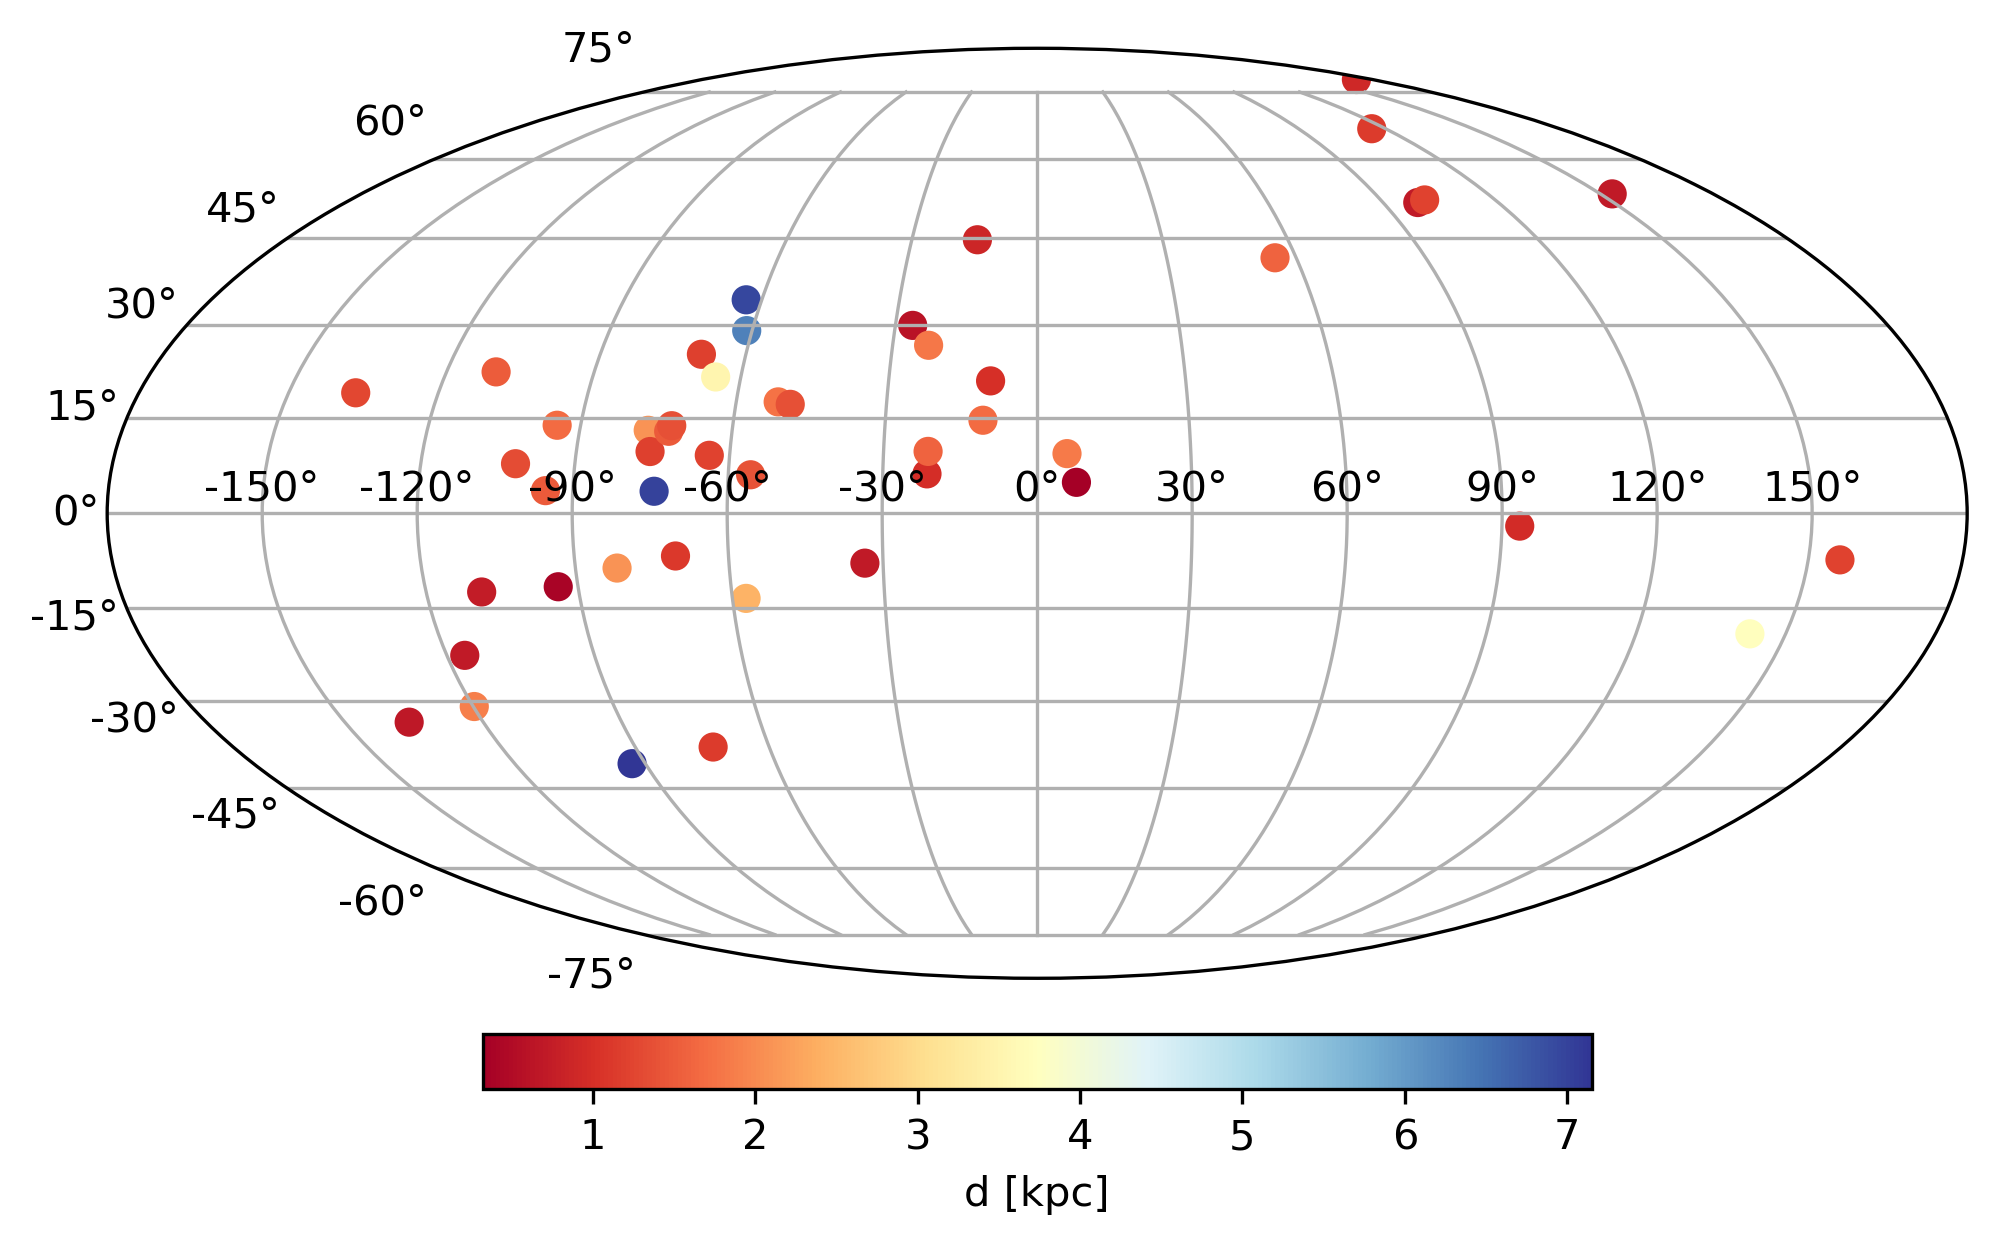
\includegraphics[width=0.8\columnwidth]{images/pulsars}
	\caption{Spatial distribution and distances of NANOGrav pulsars}
	\label{fig:pulsar_distrib}
\end{figure}




\section{Methods}


There are two potential methods we can take

\begin{enumerate}
	\item Let the states just be the frequencies $\bar{x} = (f)$. We have a linear equation for both the state evolution and the measurement matrix. Both of these depend on the parameters $\theta$. Use the likelihood output by a standard Kalman filter to run a nested sampler and try to recover $\theta$.
	\item Let the states be the frequencies and all the unknown parameters $\bar{x} = (f, \bar{\theta}_{\rm GW},\bar{\theta}_{\rm PSR},\bar{\theta}_{\rm noise})$. Our state evolution is now linear but our measurement matrix is non-linear - a function of the states(parameters). Use a non-linear estimator such as a EKF/UKF to try to recover all of the states at once.
\end{enumerate}


\subsection{Method 1}


In the case where the states are just the intrinsic pulsar frequencies, we can write the ODEs in matrix form as
\begin{equation}
	d\bar{X} = \bar{A} \bar{X} dt + \bar{N}(t) dt + \bar{\Sigma} d\bar{B}(t) 
\end{equation}
where $\bar{A} = \text{diag}(\gamma_1, \gamma_2,...)$,  $\bar{X} = \text{diag}(f_1, f_2,...)$, $\bar{N} =\text{diag}(\gamma_1[a_1+b_1t] + b_1, ...)$
and we have let $a = f_{EM}(0)$, $b = \dot{f}_{\rm EM}(0)$.


\subsection{References}
\label{sec:ref_list}





\bibliographystyle{mnras}
\bibliography{example} % if your bibtex file is called example.bib





%%%%%%%%%%%%%%%%%%%%%%%%%%%%%%%%%%%%%%%%%%%%%%%%%%


% Don't change these lines
\bsp	% typesetting comment
\label{lastpage}
\end{document}

% End of mnras_guide.tex
